%----------------------------------------------------------------------------
%----------------------------------------------------------------------------
%				    	SETUP
%----------------------------------------------------------------------------
%----------------------------------------------------------------------------

\documentclass[11pt]{article}

%----------------------------------------------------------------------------
%			  	   PACKAGES
%----------------------------------------------------------------------------

%%%%%%%%%%%%%%%%%%%%%%%
% 	  Packages
%%%%%%%%%%%%%%%%%%%%%%%

%% Fonts and Symbols
%% --------------------------
\usepackage{
	amsmath,			% math operators
	amssymb,			% math symbols
%	amsthm,				% theorem environment
	soul,				% strike through with \st{}
	xcolor,				% color!
%	xfrac,				% fancy fractions
}	

\definecolor{mygreen}{rgb}{0,0.6,0}
\definecolor{mygray}{rgb}{0.5,0.5,0.5}
\definecolor{mymauve}{rgb}{0.58,0,0.82}
\definecolor{darkblue}{rgb}{0,0,0.4}	

%% Graphics
%% --------------------
\usepackage{
	graphicx,			% allows insertion of images
	subfigure,			% allows subfigures (a), (b), etc.
	tikz,				% pretty pictures
}				
\graphicspath{ {graphics/} }	% (graphicx) relative path to graphics folder	
\usetikzlibrary{arrows, automata, calc, matrix}			

%% Tables
%% --------------------------
\usepackage{
	booktabs,			% better tables, discourages vertical rulings
	multicol,			% allow multi columns
%			tocloft,			% finer control over TOC; enabled below due to subfigure conflict
}
%\usepackage[subfigure]{tocloft}
%\addtocontents{toc}{\cftpagenumbersoff{subsubsection}} % turn off subsubsection page numbers in ToC

%% Layout Alteration
%% --------------------------
\usepackage{			
%	caption,			% line breaks in captions with \\
%	changepage,			% change margins for PARTS of pages with (adjustwidth)
	fancyhdr,			% see config in LAYOUT AND STYLING
%	floatrow,			% multiple graphics, tables, etc in figure environment
	framed,				% nice boxes; used in Supervisor's Approval
%	fullpage,			% set full page margins
	geometry,			% change the margins for specific PAGES
%	lastpage,			% used with (fancyhdr)
	parskip,			% disable indents
	pdflscape,			% ???
	rotating,			% sideways figures
}
\geometry{						% specify page size options for (geometry)
	a4paper, 			% paper size
	hmargin=1in,		% horizontal margins
	vmargin=1in,		% vertical margins
}	


%% Units
%% --------------------------
\usepackage{
	siunitx,			% has S (decimal align) column type
}
\sisetup{input-symbols = {()},  % do not treat "(" and ")" in any special way
	group-digits  = false, 	% no grouping of digits
%	load-configurations = abbreviations,
%	per-mode = symbol,
}

%% Misc
%% --------------------------
\usepackage{
	enumitem,			% better control of enumerations, descriptions, etc
	listings,			% source code import and display
}

\lstset{ %
	language=verilog,				% the language of the code
	basicstyle=\footnotesize,       % the size of the fonts that are used for the code
	numbers=none,                   % where to put the line-numbers
	numberstyle=\tiny\color{mygray},% the style that is used for the line-numbers
	stepnumber=1,                   % the step between two line-numbers. If it's 1, each line
									% 	will be numbered
	numbersep=5pt,                  % how far the line-numbers are from the code
	backgroundcolor=\color{white},  % choose the background color. You must add \usepackage{color}
	showspaces=false,               % show spaces adding particular underscores
	showstringspaces=false,         % underline spaces within strings
	showtabs=false,                 % show tabs within strings adding particular underscores
	frame=single,	                % box the code [single, none]
	rulecolor=\color{black},        % if not set, the frame-color may be changed on line-breaks
									% 	within not-black text (e.g. commens (green here))
	tabsize=2,                      % sets default tabsize to 2 spaces
	captionpos=b,                   % sets the caption-position to bottom
	breaklines=true,                % sets automatic line breaking
	breakatwhitespace=false,        % sets if automatic breaks should only happen at whitespace
	title=\lstname,                 % show the filename of files included with \lstinputlisting;
									% 	also try caption instead of title
	keywordstyle=[1]\bfseries\color{darkblue},    % keyword style for mnemonics
	keywordstyle=[2]\bfseries\color{violet},	% keyword style for . mnemonics
	commentstyle=\color{mygreen},   % comment style
	stringstyle=\color{mymauve},    % string literal style
	escapeinside={\%*}{*)},         % if you want to add a comment within your code
	morekeywords={*,...}           	% if you want to add more keywords to the set
}

%----------------------------------------------------------------------------
%		     MACROS AND COMMANDS
%----------------------------------------------------------------------------

% Defines a new command for the horizontal lines, change thickness here
\newcommand{\HRule}{\rule{\linewidth}{0.5mm}} 

% override S column type with centered text column
\newcommand{\textcol}[1]{\multicolumn{1}{c}{#1}}


% Karnaugh maps! 
% http://tex.stackexchange.com/questions/140567/drawing-karnaughs-maps-in-latex
%isolated term
%#1 - Optional. Space between node and grouping line. Default=0
%#2 - node
%#3 - filling color
\newcommand{\implicantsol}[3][0]{
	\draw[rounded corners=3pt, fill=#3, opacity=0.3] ($(#2.north west)+(135:#1)$) rectangle ($(#2.south east)+(-45:#1)$);
}


%internal group
%#1 - Optional. Space between node and grouping line. Default=0
%#2 - top left node
%#3 - bottom right node
%#4 - filling color
\newcommand{\implicant}[4][0]{
	\draw[rounded corners=3pt, fill=#4, opacity=0.3] ($(#2.north west)+(135:#1)$) rectangle ($(#3.south east)+(-45:#1)$);
}

%group lateral borders
%#1 - Optional. Space between node and grouping line. Default=0
%#2 - top left node
%#3 - bottom right node
%#4 - filling color
\newcommand{\implicantlateral}[4][0]{
	\draw[rounded corners=3pt, fill=#4, opacity=0.3] ($(rf.east |- #2.north)+(90:#1)$)-| ($(#2.east)+(0:#1)$) |- ($(rf.east |- #3.south)+(-90:#1)$);
	\draw[rounded corners=3pt, fill=#4, opacity=0.3] ($(cf.west |- #2.north)+(90:#1)$) -| ($(#3.west)+(180:#1)$) |- ($(cf.west |- #3.south)+(-90:#1)$);
}

%group top-bottom borders
%#1 - Optional. Space between node and grouping line. Default=0
%#2 - top left node
%#3 - bottom right node
%#4 - filling color
\newcommand{\implicanttopbottom}[4][0]{
	\draw[rounded corners=3pt, fill=#4, opacity=0.3] ($(cf.south -| #2.west)+(180:#1)$) |- ($(#2.south)+(-90:#1)$) -| ($(cf.south -| #3.east)+(0:#1)$);
	\draw[rounded corners=3pt, fill=#4, opacity=0.3] ($(rf.north -| #2.west)+(180:#1)$) |- ($(#3.north)+(90:#1)$) -| ($(rf.north -| #3.east)+(0:#1)$);
}

%group corners
%#1 - Optional. Space between node and grouping line. Default=0
%#2 - filling color
\newcommand{\implicantcorners}[2][0]{
	\draw[rounded corners=3pt, opacity=.3] ($(rf.east |- 0.south)+(-90:#1)$) -| ($(0.east |- cf.south)+(0:#1)$);
	\draw[rounded corners=3pt, opacity=.3] ($(rf.east |- 8.north)+(90:#1)$) -| ($(8.east |- rf.north)+(0:#1)$);
	\draw[rounded corners=3pt, opacity=.3] ($(cf.west |- 2.south)+(-90:#1)$) -| ($(2.west |- cf.south)+(180:#1)$);
	\draw[rounded corners=3pt, opacity=.3] ($(cf.west |- 10.north)+(90:#1)$) -| ($(10.west |- rf.north)+(180:#1)$);
	\fill[rounded corners=3pt, fill=#2, opacity=.3] ($(rf.east |- 0.south)+(-90:#1)$) -|  ($(0.east |- cf.south)+(0:#1)$) [sharp corners] ($(rf.east |- 0.south)+(-90:#1)$) |-  ($(0.east |- cf.south)+(0:#1)$) ;
	\fill[rounded corners=3pt, fill=#2, opacity=.3] ($(rf.east |- 8.north)+(90:#1)$) -| ($(8.east |- rf.north)+(0:#1)$) [sharp corners] ($(rf.east |- 8.north)+(90:#1)$) |- ($(8.east |- rf.north)+(0:#1)$) ;
	\fill[rounded corners=3pt, fill=#2, opacity=.3] ($(cf.west |- 2.south)+(-90:#1)$) -| ($(2.west |- cf.south)+(180:#1)$) [sharp corners]($(cf.west |- 2.south)+(-90:#1)$) |- ($(2.west |- cf.south)+(180:#1)$) ;
	\fill[rounded corners=3pt, fill=#2, opacity=.3] ($(cf.west |- 10.north)+(90:#1)$) -| ($(10.west |- rf.north)+(180:#1)$) [sharp corners] ($(cf.west |- 10.north)+(90:#1)$) |- ($(10.west |- rf.north)+(180:#1)$) ;
}

%Empty Karnaugh map 4x4
\newenvironment{Karnaugh4x4}[2]%
{
	\begin{tikzpicture}[baseline=(current bounding box.north),scale=0.8]
	\draw (0,0) grid (4,4);
	\draw (0,4) -- node [pos=0.7,above right,anchor=south west] {#2} node [pos=0.7,below left,anchor=north east] {#1} ++(135:1);
	%
	\matrix (mapa) [matrix of nodes,
	column sep={0.8cm,between origins},
	row sep={0.8cm,between origins},
	every node/.style={minimum size=0.3mm},
	anchor=8.center,
	ampersand replacement=\&] at (0.5,0.5)
	{
		\& |(c00)| 00         \& |(c01)| 01         \& |(c11)| 11         \& |(c10)| 10         \& |(cf)| \phantom{00} \\
		|(r00)| 00             \& |(0)|  \phantom{0} \& |(1)|  \phantom{0} \& |(3)|  \phantom{0} \& |(2)|  \phantom{0} \&                     \\
		|(r01)| 01             \& |(4)|  \phantom{0} \& |(5)|  \phantom{0} \& |(7)|  \phantom{0} \& |(6)|  \phantom{0} \&                     \\
		|(r11)| 11             \& |(12)| \phantom{0} \& |(13)| \phantom{0} \& |(15)| \phantom{0} \& |(14)| \phantom{0} \&                     \\
		|(r10)| 10             \& |(8)|  \phantom{0} \& |(9)|  \phantom{0} \& |(11)| \phantom{0} \& |(10)| \phantom{0} \&                     \\
		|(rf) | \phantom{00}   \&                    \&                    \&                    \&                    \&                     \\
	};
}%
{
	\end{tikzpicture}
}

%Empty Karnaugh map 2x4
\newenvironment{Karnaugh2x4}[2]%
{
	\begin{tikzpicture}[baseline=(current bounding box.north),scale=0.8]
	\draw (0,0) grid (4,2);
	\draw (0,2) -- node [pos=0.7,above right,anchor=south west] {#2} node [pos=0.7,below left,anchor=north east] {#1} ++(135:1);
	%
	\matrix (mapa) [matrix of nodes,
	column sep={0.8cm,between origins},
	row sep={0.8cm,between origins},
	every node/.style={minimum size=0.3mm},
	anchor=4.center,
	ampersand replacement=\&] at (0.5,0.5)
	{
		\& |(c00)| 00         \& |(c01)| 01         \& |(c11)| 11         \& |(c10)| 10         \& |(cf)| \phantom{00} \\
		|(r00)| 0             \& |(0)|  \phantom{0} \& |(1)|  \phantom{0} \& |(3)|  \phantom{0} \& |(2)|  \phantom{0} \&                     \\
		|(r01)| 1             \& |(4)|  \phantom{0} \& |(5)|  \phantom{0} \& |(7)|  \phantom{0} \& |(6)|  \phantom{0} \&                     \\
		|(rf) | \phantom{00}  \&                    \&                    \&                    \&                    \&                     \\
	};
}%
{
	\end{tikzpicture}
}

%Empty Karnaugh map 2x2
\newenvironment{Karnaugh2x2}[2]%
{
	\begin{tikzpicture}[baseline=(current bounding box.north),scale=0.8]
	\draw (0,0) grid (2,2);
	\draw (0,2) -- node [pos=0.7,above right,anchor=south west] {#2} node [pos=0.7,below left,anchor=north east] {#1} ++(135:1);
	%
	\matrix (mapa) [matrix of nodes,
	column sep={0.8cm,between origins},
	row sep={0.8cm,between origins},
	every node/.style={minimum size=0.3mm},
	anchor=2.center,
	ampersand replacement=\&] at (0.5,0.5)
	{
		\& |(c00)| 0          \& |(c01)| 1  \\
		|(r00)| 0 \& |(0)|  \phantom{0} \& |(1)|  \phantom{0} \\
		|(r01)| 1 \& |(2)|  \phantom{0} \& |(3)|  \phantom{0} \\
	};
}%
{
	\end{tikzpicture}
}

%Defines 8 or 16 values (0,1,X)
\newcommand{\contingut}[1]{%
	\foreach \x [count=\xi from 0]  in {#1}
	\path (\xi) node {\x};
}

%Places 1 in listed positions
\newcommand{\minterms}[1]{%
	\foreach \x in {#1}
	\path (\x) node {1};
}

%Places 0 in listed positions
\newcommand{\maxterms}[1]{%
	\foreach \x in {#1}
	\path (\x) node {0};
}

%Places X in listed positions
\newcommand{\dontcare}[1]{%
	\foreach \x in {#1}
	\path (\x) node {X};
}


%----------------------------------------------------------------------------
%----------------------------------------------------------------------------
%				   DOCUMENT
%----------------------------------------------------------------------------
%----------------------------------------------------------------------------

\begin{document}

%----------------------------------------------------------------------------
%				    TITLE PAGE
%----------------------------------------------------------------------------

\begin{titlepage}

\center
 
% Header
\textsc{\LARGE University of Victoria}\\[1cm] 	% Name of your university/college
\textsc{\Large CENG 241}\\[0.5cm] 			% Major heading such as course name
\textsc{\large Digital Design I}\\[0.5cm] 		% Minor heading such as course title


% Lab Title
\HRule \\[0.4cm]
{\huge \bfseries Lab 6 \\ Finite state machines: \\Mealy and Moore circuits}\\[0.2cm] % Title of your document
\HRule \\[1.5cm]
 
 
%Lab Instructor Details
\begin{minipage}{0.7\textwidth}
\begin{flushleft} 

\large\emph{Instructor:} \\
Dr. Amirali \textsc{Baniasadi} \\
\vspace{12 pt}
\emph{Teaching Assistant:} \\
Grace \textsc{Hui}

\end{flushleft}
\end{minipage}
~
%% No content here, but it keeps the alignment of the instructor/TA
%% box correct.
%% Consider revising.
\begin{minipage}{0.1\textwidth}
\begin{flushright} \large
%Dr. Barbara \textsc{Sawicka} \\
\vspace{12 pt}
%\emph{Teaching Assistant:} \\
%Vahid \textsc{Moradi}
\end{flushright}
\end{minipage}\\[2cm]


% Lab members
\Large Yves \textsc{S\'{e}n\'{e}chal}
\large V00213837	\\
\Large Tyler \textsc{Stephen}
\large V00812021	\\
A01 - B03\\[1.5cm] 


% Date
{\large July 13, 2015}\\ % Date, change the \today to a set date if you want to be precise

% Logo
\begin{figure}[b]	 % put logo at bottom of the page
	\centering
	\includegraphics[scale=0.3]{UVic_logo}
\end{figure}

\end{titlepage}

%----------------------------------------------------------------------------
%				    BODY
%----------------------------------------------------------------------------

\section{Introduction}
This lab will explore the difference between Mealy and Moore state machines. Both types of state machine will be constructed to detect a specific input sequence. The entire design process will be demonstrated for both machines.

\section{Discussion}\label{sec:discussion}
%{\em A brief description about what the circuit will do.
%	
%	Difference between Moore and Mealy?
%	
%	Method for generating circuits? State machine $\rightarrow$ Truth table $\rightarrow$ Kmap $\rightarrow$ Boolean $\rightarrow$ circuits}

Suppose we want to detect the sequence ``1101'' within an input stream. Overlapping sequences will be detect (i.e. the last 1 of the first sequence can be the first 1 of the next sequence). The input and output will follow this pattern:

\begin{table}[htpb]
	\centering
	\begin{tabular}{l c}
		Input & 1001\;1011\;0100\;1101 \\
		Output & 0000\;0010\;0100\;0001 \\
	\end{tabular}
\end{table}

It is possible to design a sequential circuit to accomplish this task. First, the system's response to input will be codified into a state diagram. Next, this state diagram will be translated into state tables. From there, Karnaugh maps and Boolean expressions will inform the physical design of the circuit.

\subsection{State diagrams}
There are two types of state machine to choose from: the Moore machine and the Mealy machine. The Moore machine can determine its output based entirely on the current state. The Mealy machine needs to know the input in addition to the current state to determine its output. Since Mealy machines link the output to the input for a state, they will always require the same or fewer states than the equivalent Moore machine.

Figure \ref{fig:state_machines} shows both state diagrams for the sequence detector. Overlapping sequence detection is controlled by having the final 1 input link to the ``interior'' of the state diagram rather than the initial state.

\begin{figure}[htpb]
	\centering
	\subfigure[Moore machine]
	{
		\begin{tikzpicture}
		[>=stealth',shorten >=1pt,auto,node distance=3cm]
		\node[initial,state] (a)				{$a/0$};
		\node[state]         (b) [right of=a]	{$b/0$};
		\node[state]         (c) [right of=b] 	{$c/0$};
		\node[state]         (d) [right of=c] 	{$d/0$};
		\node[state]         (e) [right of=d] 	{$e/1$};
		
		\path[->] 
		(a)	edge [loop above] 	node 		 	{0} (a)
			edge              	node 		 	{1} (b)
		(b) edge [bend left]  	node [pos=0.3]	{0} (a)
			edge              	node 		 	{1} (c)
		(c) edge [bend left=40]	node [pos=0.48]	{1} (a)
			edge			  	node 			{0} (d)
		(d) edge [bend left=50]	node 		 	{0} (a)
			edge 			  	node 		 	{1} (e)
		(e) edge [bend right=40]node [above] 	{0} (a)
			edge [bend right]  	node [above] 	{1} (c);
		\end{tikzpicture}
	}
	\subfigure[Mealy machine]
	{
		\begin{tikzpicture}
		[>=stealth',shorten >=1pt,auto,node distance=3cm]
		\node[initial,state] (a)				{$a$};
		\node[state]         (b) [right of=a]	{$b$};
		\node[state]         (c) [right of=b] 	{$c$};
		\node[state]         (d) [right of=c] 	{$d$};
		
		\path[->] 
		(a)	edge [loop above] 	node 		 	{$0/0$} (a)
			edge              	node 		 	{$1/0$} (b)
		(b) edge [bend left]  	node [pos=0.3]	{$0/0$} (a)
			edge              	node 		 	{$1/0$} (c)
		(c) edge [bend left=40]	node [pos=0.48]	{$1/0$} (a)
			edge			  	node 			{$0/0$} (d)
		(d) edge [bend right=50]node [above] 	{$0/0$} (a)
			edge [bend right=35]node [above] 	{$1/1$} (b);
		\end{tikzpicture}
	}
	\caption{State machines to detect sequence ``1101'' with overlap}
	\label{fig:state_machines}
\end{figure}

\pagebreak
\subsection{Transition tables}
To create the state transition tables, first enumerate the states. The number of flip-flops required will be equal to $\lceil \log_2 \left( \text{number of states} \right) \rceil$. The next state is determined by following the state diagram. For the output, the Mealy transition table requires the input in addition to the current state. D flip-flops were used to construct the circuits in this lab. Consequently, the results of the next state table can be used directly as inputs for the flip-flops. The next state table will require an accompanying excitation table for T or JK flip-flops.
\begin{figure}[htpb]
	\centering
	\subfigure[State enumeration]
	{
		\begin{tabular}{c | c c c }
			State & $S_2$ & $S_1$ & $S_0$ \\
			\hline
			$a$ & 0 & 0 & 0 \\
			$b$ & 0 & 0 & 1 \\
			$c$ & 0 & 1 & 0 \\
			$d$ & 0 & 1 & 1 \\
			$e$ & 1 & 0 & 0 \\
			 -  & 1 & 0 & 1 \\
			 -  & 1 & 1 & 0 \\
			 -  & 1 & 1 & 1 \\
		\end{tabular}
	}
	\subfigure[Next state]
	{
		\begin{tabular}{c c c c | c c c}
			$S_2$ & $S_1$ & $S_0$ & $X$ & $S_2^+$ & $S_1^+$ & $S_0^+$ \\
			\hline
			0 & 0 & 0 & 0 & 0 & 0 & 0 \\
			0 & 0 & 0 & 1 & 0 & 0 & 1 \\
			0 & 0 & 1 & 0 & 0 & 0 & 0 \\
			0 & 0 & 1 & 1 & 0 & 1 & 0 \\
			0 & 1 & 0 & 0 & 0 & 1 & 1 \\
			0 & 1 & 0 & 1 & 0 & 0 & 0 \\
			0 & 1 & 1 & 0 & 0 & 0 & 0 \\
			0 & 1 & 1 & 1 & 1 & 0 & 0 \\
			1 & 0 & 0 & 0 & 0 & 0 & 0 \\
			1 & 0 & 0 & 1 & 0 & 1 & 0 \\
			1 & 0 & 1 & 0 & - & - & - \\
			1 & 0 & 1 & 1 & - & - & - \\
			1 & 1 & 0 & 0 & - & - & - \\
			1 & 1 & 0 & 1 & - & - & - \\
			1 & 1 & 1 & 0 & - & - & - \\
			1 & 1 & 1 & 1 & - & - & - \\
		\end{tabular}
	}
	\subfigure[Output]
	{
		\begin{tabular}{c c c | c }
			$S_2$ & $S_1$ & $S_0$ & $Z$ \\
			\hline
			0 & 0 & 0 & 0 \\
			0 & 0 & 1 & 0 \\
			0 & 1 & 0 & 0 \\
			0 & 1 & 1 & 0 \\
			1 & 0 & 0 & 1 \\
			1 & 0 & 1 & - \\
			1 & 1 & 0 & - \\
			1 & 1 & 1 & - \\
		\end{tabular}
	}
	\caption[figurename=Table]{Transition tables for the Moore machine}
	\label{table:transition-mealy}
\end{figure}

\begin{figure}[htpb]
	\centering
	\subfigure[State enumeration]
	{
		\begin{tabular}{c | c c}
			State & $S_0$ & $S_1$ \\
			\hline
			$a$ & 0 & 0 \\
			$b$ & 0 & 1 \\
			$c$ & 1 & 0 \\
			$d$ & 1 & 1 \\
		\end{tabular}
	}
	\subfigure[Next state]
	{
		\begin{tabular}{ c c c | c c}
			$S_1$ & $S_0$ & $X$ & $S_1^+$ & $S_0^+$ \\
			\hline
			0 & 0 & 0 & 0 & 0 \\
			0 & 0 & 1 & 0 & 1 \\
			0 & 1 & 0 & 0 & 0 \\
			0 & 1 & 1 & 1 & 0 \\
			1 & 0 & 0 & 1 & 1 \\
			1 & 0 & 1 & 0 & 0 \\
			1 & 1 & 0 & 0 & 0 \\
			1 & 1 & 1 & 0 & 1 \\
		\end{tabular}
	}
	\subfigure[Output]
	{
		\begin{tabular}{ c c c | c }
			$S_1$ & $S_0$ & $X$ & $Z$ \\
			\hline
			0 & 0 & 0 & 0 \\
			0 & 0 & 1 & 0 \\
			0 & 1 & 0 & 0 \\
			0 & 1 & 1 & 0 \\
			1 & 0 & 0 & 0 \\
			1 & 0 & 1 & 0 \\
			1 & 1 & 0 & 0 \\
			1 & 1 & 1 & 1 \\
		\end{tabular}
	}
	\caption[figurename=Table]{Transition tables for the Mealy machine}
	\label{table:transition_mealy}
\end{figure}

\newpage
\subsection{Karnaugh maps}
Karnaugh maps are generated from the transition tables. The Moore and Mealy methods are identical from this point in the design going forward.
\begin{figure}[htpb]
	\centering
	\subfigure[$S_2^+$]
	{
		\begin{Karnaugh4x4}{$S_2 S_1$}{$S_0 X$}
			\minterms{7}
			\maxterms{0, 1, 2, 3, 4, 5, 6, 8, 9}
			\dontcare{10, 11, 12, 13, 14, 15}
			\implicant{7}{15}{gray}			
		\end{Karnaugh4x4}
	}
	\subfigure[$S_1^+$]
	{
		\begin{Karnaugh4x4}{$S_2 S_1$}{$S_0 X$}
			\minterms{3, 4, 9}
			\maxterms{0, 1, 2, 5, 6, 7, 8}
			\dontcare{10, 11, 12, 13, 14, 15}
			\implicant{4}{12}{gray}
			\implicanttopbottom{3}{11}{gray}
			\implicant{13}{11}{gray}
		\end{Karnaugh4x4}
	}
	\subfigure[$S_0^+$]
	{
		\begin{Karnaugh4x4}{$S_2 S_1$}{$S_0 X$}
			\minterms{1, 4, 9}
			\maxterms{0, 2, 3, 5, 6, 7, 8}
			\dontcare{10, 11, 12, 13, 14, 15}
			\implicant{4}{12}{gray}
			\implicanttopbottom{1}{9}{gray}
		\end{Karnaugh4x4}
	}
	\subfigure[$Z$]
	{
		\begin{Karnaugh2x4}{$S_2$}{$S_1 S_0$}
			\minterms{4}
			\maxterms{0, 1, 2, 3}
			\dontcare{5, 6, 7}
			\implicant{4}{6}{gray}
		\end{Karnaugh2x4}
	}
	\caption{Karnaugh maps for the Moore machine}
\end{figure}

The optimal boolean functions for the Moore machine are
\begin{align*}
S_2^+ &= S_1 S_0 X \\	
S_1^+ &= S_1 S_0^\prime X^\prime + S_1^\prime S_0 X + S_2 X \\
S_0^+ &= S_1 S_0^\prime X^\prime + S_1^\prime S_0^\prime X \\
Z &= S_2
\end{align*}

\newpage
\begin{figure}[htpb]
	\centering
	\subfigure[$S_1^+$]
	{
		\begin{Karnaugh2x4}{$S_1$}{$S_0 X$}
			\minterms{3, 4}
			\maxterms{0, 1, 2, 5, 6, 7}
			\implicantsol{3}{gray}
			\implicantsol{4}{gray}
		\end{Karnaugh2x4}	
	}
	\subfigure[$S_0^+$]
	{
		\begin{Karnaugh2x4}{$S_1$}{$S_0 X$}
			\minterms{1, 4, 7}
			\maxterms{0, 2, 3, 5, 6}
			\implicantsol{1}{gray}
			\implicantsol{4}{gray}
			\implicantsol{7}{gray}
		\end{Karnaugh2x4}	
	}
	\subfigure[$Z$]
	{
		\begin{Karnaugh2x4}{$S_1$}{$S_0 X$}
			\minterms{7}
			\maxterms{0, 1, 2, 3, 4, 5, 6}
			\implicantsol{7}{gray}
		\end{Karnaugh2x4}	
	}
	\caption{Karnaugh maps for the Mealy machine}
	\label{fig:kmaps}
\end{figure}

The optimal boolean functions for the Mealy machine are
\begin{align*}
	S_1^+ &= S_1 S_0^\prime X^\prime + S_1^\prime S_0 X \\
	S_0^+ &= S_1 S_0^\prime X^\prime + S_1^\prime S_0^\prime X + S_1 S_0 X\\
		Z &= S_1 S_0 X\\
\end{align*}

\section{Simulations}
%{\em Include schematic for Mealy machine and functional output}

We chose to construct the Mealy machine because it required one fewer flip-flop. The Boolean expression was implemented in the schematic in Figure \ref{fig:schematic}.

\begin{figure}[tbph]
\centering
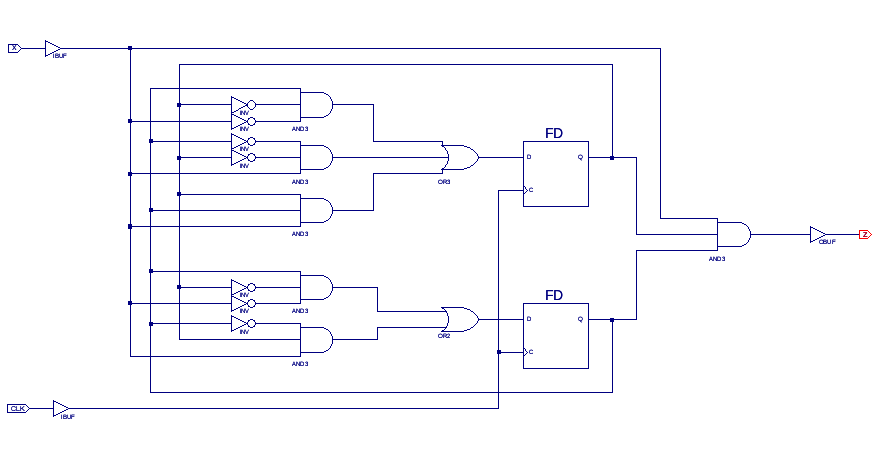
\includegraphics[width=0.95\linewidth]{graphics/lab6_schematic}
\caption{Mealy machine schematic}
\label{fig:schematic}
\end{figure}

The input stream from the beginning of Section \ref{sec:discussion} was used as a simulation input source. Figure \ref{fig:sim} shows that the schematic gives the correct output in a Xilinx simulation.

\begin{figure}[tbph]
\centering
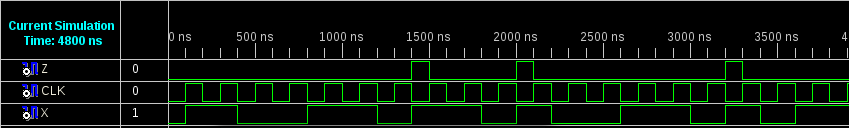
\includegraphics[width=0.95\linewidth]{graphics/lab6_simulation}
\caption{The Mealy machine correctly identifies the sequence ``1101'' from the input stream}
\label{fig:sim}
\end{figure}

The schematics were used to construct a Mealy machine using physical ICs. It was also successful in identifying the sequence from the input stream.

\section{Conclusion}
Sequential circuits can be created from Moore and Mealy machines. We were successful in creating a sequence detecting machine using the Mealy method and confirmed the results with computer and physical simulations.

\end{document}